%% ---------------------------- SOFTWARE AND OS IMPLEMENTATION ----------------------------
\subsection{Software and operating system implementation}
\label{s:LabEnv}
\begin{figure}[htbp]
\centerline{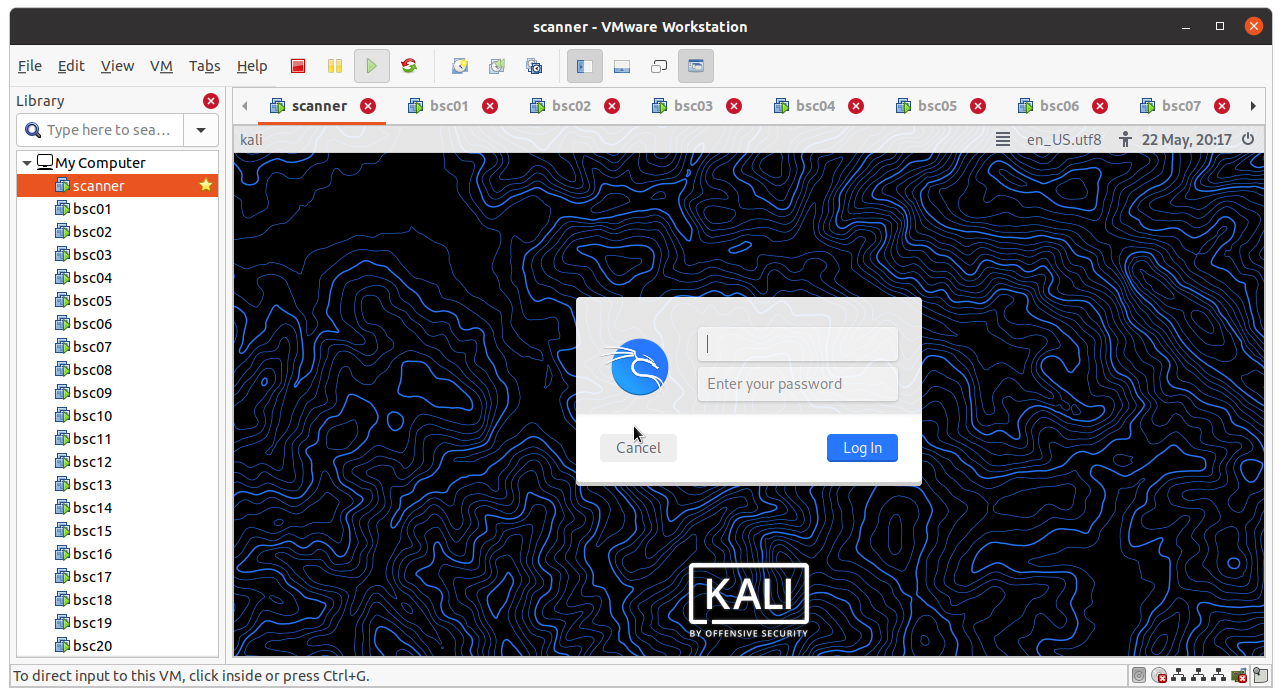
\includegraphics[scale=0.35]{images/lab/vmware-lab.png}}
\caption{Lab environment shown in VMware Workstation}
\label{fig:LabVMware}
\end{figure}

VMware Workstation 16.1 was used to set up 20 virtual hosts (referred to as workers) using Ubuntu 20.04 (Linux kernel 5.4.0-81-generic \#91) with the only target of capturing packet captures from the scanner host.
The host running the VMware Workstation is using Ubuntu Linux 20.04.4 (Linux kernel 5.13.0-35-generic \#40).
One virtual host (referred to as the scanner host) were installed with Kali Linux 2021.4 (Linux kernel 5.14.0-kali4-amd64 \#1) for conducting a various type of scans, issuing tasks to the workers, and monitoring ongoing scans.
Both these operating systems are based on Debian, which simplifies setup, configuration, and troubleshooting during the research. These operating systems are also easy to install and use without a large need for customization, which reduces the time consumption during the research as well.
